    \section{Abstract}
    The adsorption of ions to soft-porous interfaces plays a critical role in 
    many physical and biological processes, such as the function of electrochemical 
    energy storage devices or 
    the attachment of membrane proteins to cells surfaces. 
    In this work we characterize different adsorption modes, and
    describe the adsorption behavior of Na\textsuperscript{+}, Li\textsuperscript{+}, and Mg\textsuperscript{2+} 
    {onto a porous substrate}.
    We identify three categories of adsorption based on 
    the degree of dehydration of the ion, 
    viz., steric adsorption {corresponding to a lack of dehydration}, 
    imperfect adsorption {with partial dehydration}, and 
    perfect adsorption {representing total dehydration}.
    Using 1-palmitoyl-2-oleoyl-sn-glycero-3-phosphatidylcholine (POPC) 
    in salt solution as a generic model system for salt at a soft and 
    porous interface, based on the simulation model used we find that 
    anions, \cl, always adsorb sterically. Among cations, the divalent
    \mg does not dehydrate, and is {also} adsorbed sterically. 
    On the other hand, \na  
    adsorbed to a large fraction perfectly 
    {and \li{} exhibits a significant fraction of imperfectly adsorbed ions,}
    We demonstrate that, with everything else held fixed, the 
    adsorption mode of a cation is determined
    solely by the strength of the electric field produced by the 
    ion at the distance of the hydration shell. 


\section{Introduction}
Interactions of ions with soft, porous, and charge-neutral substrates
such as zwitterionic lipid bilayers are important and a common
system of interest in soft matter physics and biophysics.
Empirical studies towards these use simplified
models to interpret observations, e.g. assuming the water as a
dielectric continuum,
or taking the ions as a spherical entity surrounded
by a neatly organized hydration shell~\cite{israelachvili:2011:intermol}.

A simple way of defining adsorption of ions to a substrate 
comes from the Poission-Boltzmann (PB) theory~\cite{israelachvili:2011:intermol}.
{This mean-field approximation predicts accumulation
of ions near a surface due to the mutual electrostatic repulsion
of the ions and entropic factors.}
{Deviations in ion distribution from the predictions of PB theory near a substrate are
    the defining characteristic of the specific adsorption phenomenon
~\cite{stern:1924:theory,grahame:1947:electrical}.}

Experimental studies of ion adsorption can be broadly
classified into two main groups -- methods that examine the electric field/surface potential
produced by the adsorbed ions, e.g, electrophoretic mobility~\cite{smith:2017:zeta} or 
measurement of the forces between 
bilayers~\cite{marra:1985:direct}, and methods
that can more directly characterize the location and dynamics of ions such 
as x-ray or neutron 
scattering~\cite{fogarty:2015,nagle:2000,pan:2012,panff:2012,uhrikova:2008,mason:2006:neutron}, and
NMR~\cite{nagle:2000,venable:2013,casal:1989}. 

At the atomistic level, identifying adsorbed ions poses a different kind of challenge.
We have addressed this issue previously,
where we characterized adsorption by examining the dehydration of ions near the
interface~\cite{kruczek:2019,kruczek:2017,pandit:2003:dppc:na,Berkowitz:2006}.
This is similar to the kind of adsorption described 
by the Langmuir isotherm model, where it is
assumed that ions stick to a soft, porous interface 
through direct interaction~\cite{kalinin:1996:ionbinding}.
Adsorption defined thusly has been reported in our previous works for monovalent ions 
such as \na and {\li{}}\cite{kruczek:2017,kruczek:2019,saunders:2019,saunders:2022}.
Further, our previous work on divalent ions
exhibited that \mg maintains its 
hydration {structure} regardless of where the ion is located in the 
lipid bilayer~\cite{kruczek:2019}, yet maintaining 
a distribution distinct from that
predicted by PB theory. Hence, {in this work
    we characterize different modes of adsorption corresponding
to different ions. Here we} categorize the 
adsorption behavior based on degree of 
dehydration, starting from no
dehydration at all as in the case of \mg and Cl\textsuperscript{-}, 
extending to complete dehydration as in the case with Na\textsuperscript{+}. 
In {the somewhat different} 
context of RNA, which is not a soft, 
porous substrate, the specific binding of ions has been addressed
extensively
~\cite{bowman:2012,rulivsek:2003:outer,dudev:2003,porschke:1979:mode,petrov:2005}
based on the mobility of cations and further 
characterized by models that describe the 
structure of their coordination shell.
Cations bound to RNA are frequently distinguished as
being diffuse {(similar to our steric adsorbed case)}, and the site-bound ions are further characterized
by outer-shell {(again analogous to our steric adsorption ions)} 
or inner shell binding 
{(analogous to the imperfect or perfect adsorbed ions)}, depending on
the folded conformation of the RNA or 
nearby nucleotides~\cite{bowman:2012,rulivsek:2003:outer,dudev:2003,porschke:1979:mode,petrov:2005}. 

Along with dehydration, we use specific 
adsorption in the context of PB density 
as the defining property
of adsorption phenomenon. 
Based on our previous as well as current atomistic simulations we broadly
classify adsorption of ions into three categories -- viz. 
\emph{perfect adsorption}, \emph{imperfect adsorption},
and \emph{steric adsorption}. We also demonstrate that,
using different
force-field for \mg the predominant mode of adsorption
of \mg to 1-palmitoyl-2-oleoyl-sn-glycero-3-phosphatidylcholine (POPC) is 
{always} \emph{steric adsorption}.

\section{Methods}
We perform multiple simulations of POPC bilayers
with LiCl and MgCl$_{2}$ salt. Configurations for each simulation are listed in table~\ref{tabch3:ions}.
\begin{table}
    \caption[Simulation system details]{Simulation system details. Each simulated system is started with 200~mM salt, and the final bulk concentration 
    is computed from the average number density of ions 
    at the center of the solvent occupied region of the box, from the last 150~ns of simulation time. \nambnbfix
    simulation trajectories are published in our previous work, and are re-analyzed in this work. 
    The \mgmbnbfix system is extended to 2.5~$\mu$s to ascertain if any 
    exchange of waters from the first shell of \mg could be observed. \li{} (a) parameters are obtained from 
    the work by Joung and Chetatham III~\cite{joung:2008}. \mg (b-c) parameters
    are obtained from Li \etal{}~\cite{merzparams} and Grotz \etal{}~\cite{microparams}, respectively.}
    \label{tabch3:ions}
    \begin{minipage}{\textwidth}
    \tiny{
    \begin{tabularx}{\textwidth}{X|X|X|X|X|X}
        System & No. of Cations & No. of Anions & Starting Bulk Salt Concentration & Final Bulk Salt Concentration & Simulated Time \\\hline
        \na{\tiny{From Saunders \etal{} 2022~\cite{saunders:2022}}}      & 216  & 216   &   200mM   & 103mM & 0.7$\mu$s\\\hline
        \li{} (a)         & 216  & 216   &   200mM   & 102.0mM & 1$\mu$s  \\\hline
        \mg (b)         & 216  & 432   &   200mM   & 152mM  & 2.5$\mu$s\\\hline
        \mg (c)           & 216  & 432   &   200mM   & 153mM & 1$\mu$s\\\hline
    \end{tabularx}}\par
   \vspace{-0.75\skip\footins}
   \renewcommand{\footnoterule}{}
\end{minipage}
\end{table}
{Bilayers are constructed of 200 lipids, with 100 lipids per leaflet.}
Simulations are all performed with 
60,000 water molecules to ensure that the simulation box
was large enough to have no long-range dipole moment, 
and have a significant 
sampling of bulk water. The inclusion of ions substantially increases the region of ordered 
waters in the system~\cite{kruczek:2019,saunders:2022}.
We simulate these systems with a starting concentration of 200~mM salt, in order to ensure
that the equilibrium bulk concentration is physiologically relevant and 
{yet} statistically viable.
Systems with \mg are simulated with twice the number of 
anions to counter the +2 charge of the cation. All the systems are simulated for 1~$\mu$s of simulated time. 
The \mgmbnbfix system is extended to 2.5~$\mu$s to confirm the 
long residence time of waters in the first coordination shell of \mg\cite{grotz:2021:optimized}. 
It is observed that ions in the bilayer still do not
exchange of waters from their first coordination shell, 
so another 1~$\mu$s simulation is performed using the water-\mg 
interaction model developed by Grotz \etal{}, which significantly increase the water-exchange rate to be closer 
to the value observed experimentally~\cite{grotz:2021:optimized}.
{All the} simulations are performed using the GROMACS molecular dynamics software package, 
version 5.1.6~\cite{abraham:2015,pall:2014,van:2005,lindahl:2001,berendsen:1995}, and analysis is performed using 
GROMACS built--in analysis tools and in--house software developed
on the gromacs API or using the MDanalysis python package~\cite{gromacsmanual,mdanalysis1,mdanalysis2}.
\subsection{Bilayer Construction}

I construct the bilayers by arranging 100 POPC lipids on a $10 \times 10$ grid
and reflecting this leaflet along the $z$--axis to generate the second leaflet.
A solvent block of 60,000 waters is then added, and a subset of water molecules
is randomly replaced with ions to achieve the desired system compositions
(see Table~\ref{tabch3:ions}). 

Following energy minimization with the steepest--descents algorithm to remove
bad contacts, I relax each system with a 1~ns NPT simulation at 250~K.
Systems are then annealed by heating to 350~K and cooling in 10~K steps to the
production temperature of 300~K, with each step lasting 155~ps.
The final annealed configurations are used as the initial structures for
production molecular dynamics simulations.

\subsection{Molecular Dynamics}

Production simulations are run with lengths given in Table~\ref{tabch3:ions}.
Trajectory analysis is performed using a combination of GROMACS built--in
tools and in--house software developed on the GROMACS API.


\subsection{Force-field parameters}

Lipid-lipid and lipid-water interactions are described using our 
gromos43a1-s3 model~\cite{chiu:2009}, 
which is calibrated to work with the SPC/E water model~\cite{spce}. 
Li$^+$-water interactions 
are described using Joung and Cheatham parameters~\cite{joung:2008}. 
Target data are computed using the method described in Saunders \etal~\cite{saunders:2022} and in the first chapter of this dissertation
to compute non-aqueous cross-terms for \li{}. Target data consist of substitution
energies and optimized geometries of \li{} clusters with water, methyl acetate,
and diethyl phosphate ligands. The substitution energies from DFT calculations
serve as benchmarks for parameter optimization, and are compared against
Lorentz–Berthelot mixing rules and the optimized parameters
(see Table~\ref{tabch3:params} and Figures~\ref{figch3:energies}--\ref{figch3:distances}).

\begin{figure}
    \caption[Substitution energies of \li{} from solvent to ligands]{Substitution energies of \li{} clusters with methyl acetate and diethyl phosphate ligands.
    Black points are \emph{ab initio} values, blue is the Lorentz--Berthelot prediction, and red is the result of the optimized parameters.}
    \label{figch3:energies}
    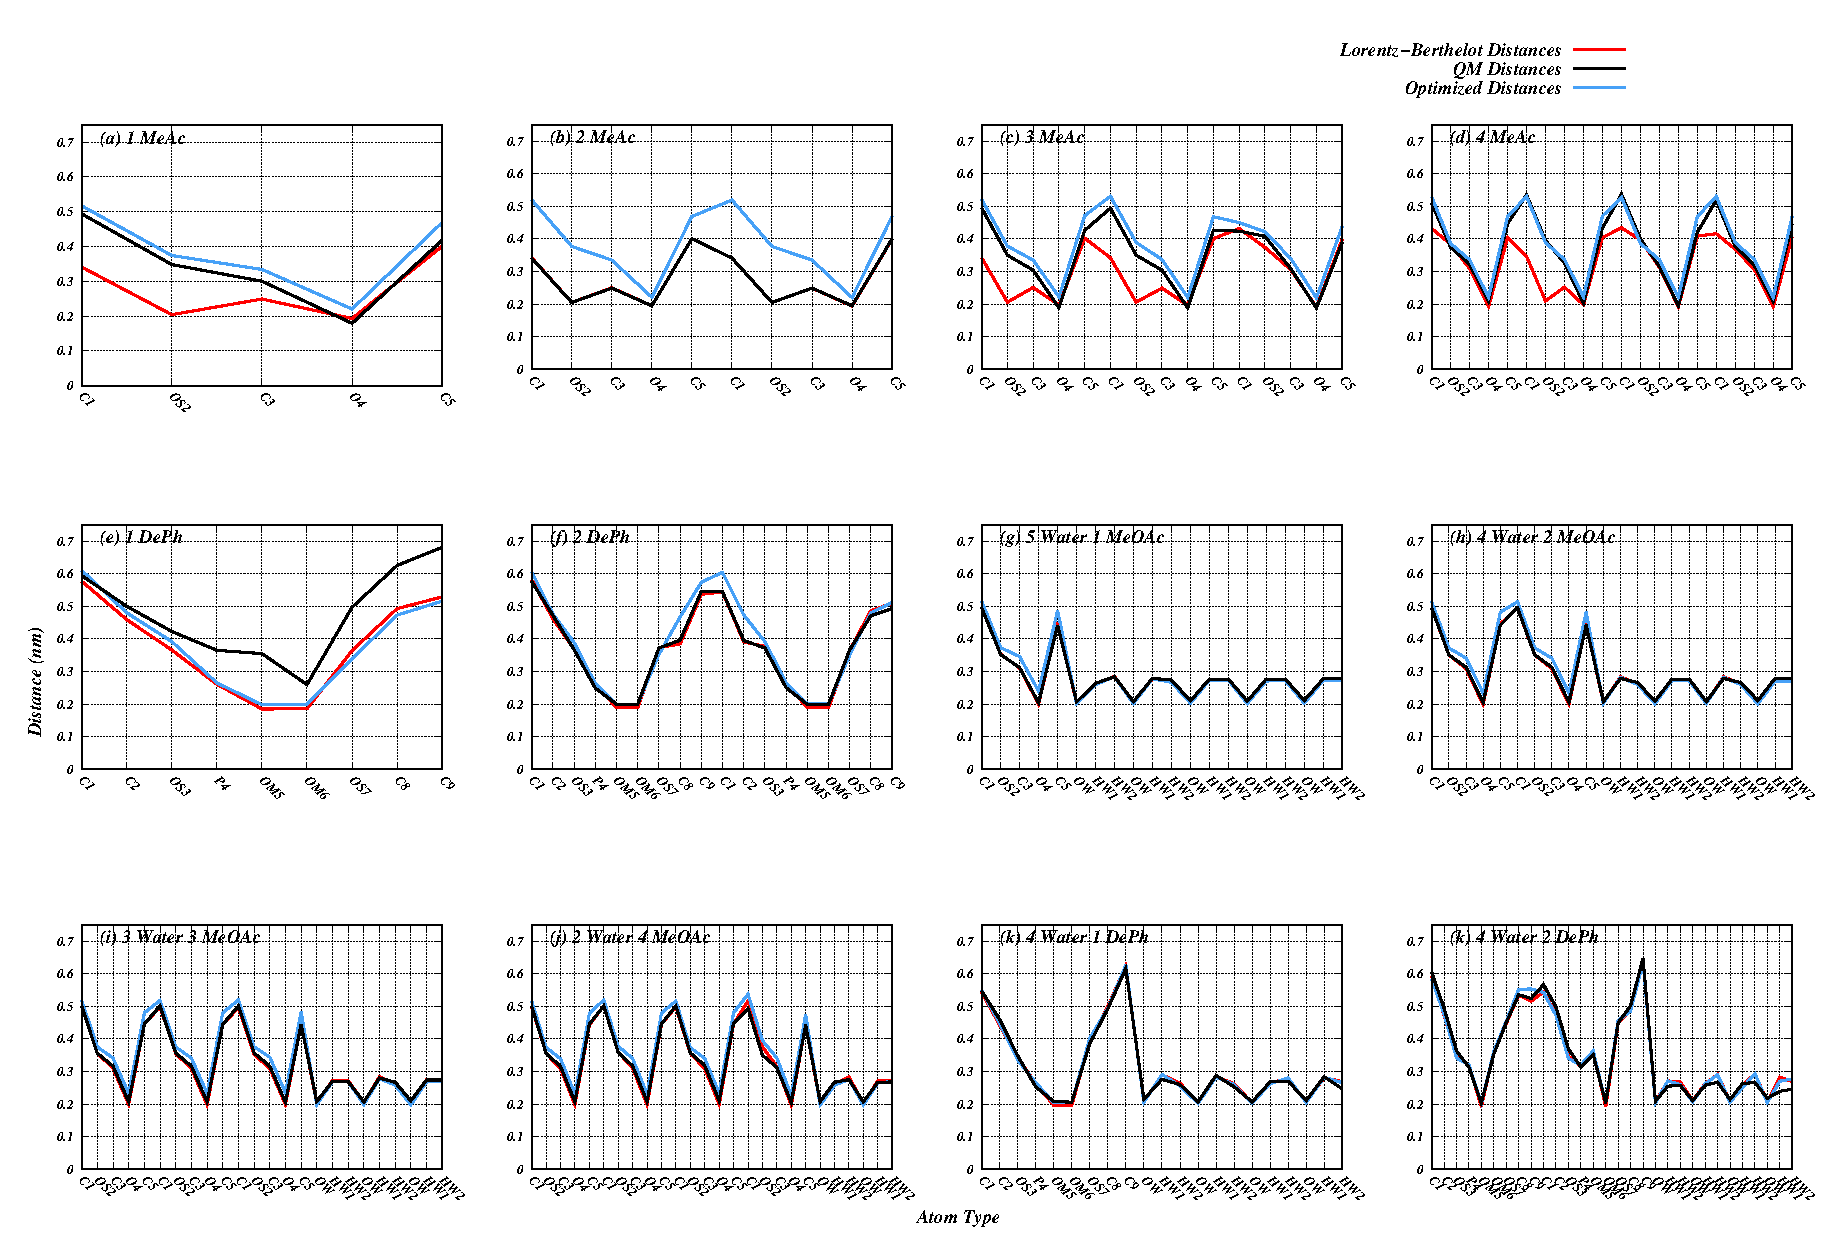
\includegraphics[width=\textwidth]{Figure_S1.eps}
\end{figure}

\begin{figure}
    \caption[Geometries of \li{} clusters with ligands]{Distances of all ligand atoms from \li{} for each cluster. 
    Lorentz--Berthelot parameters give geometries close to the target data, while the optimized parameters
    bring the ion slightly closer to electronegative oxygens.}
    \label{figch3:distances}
    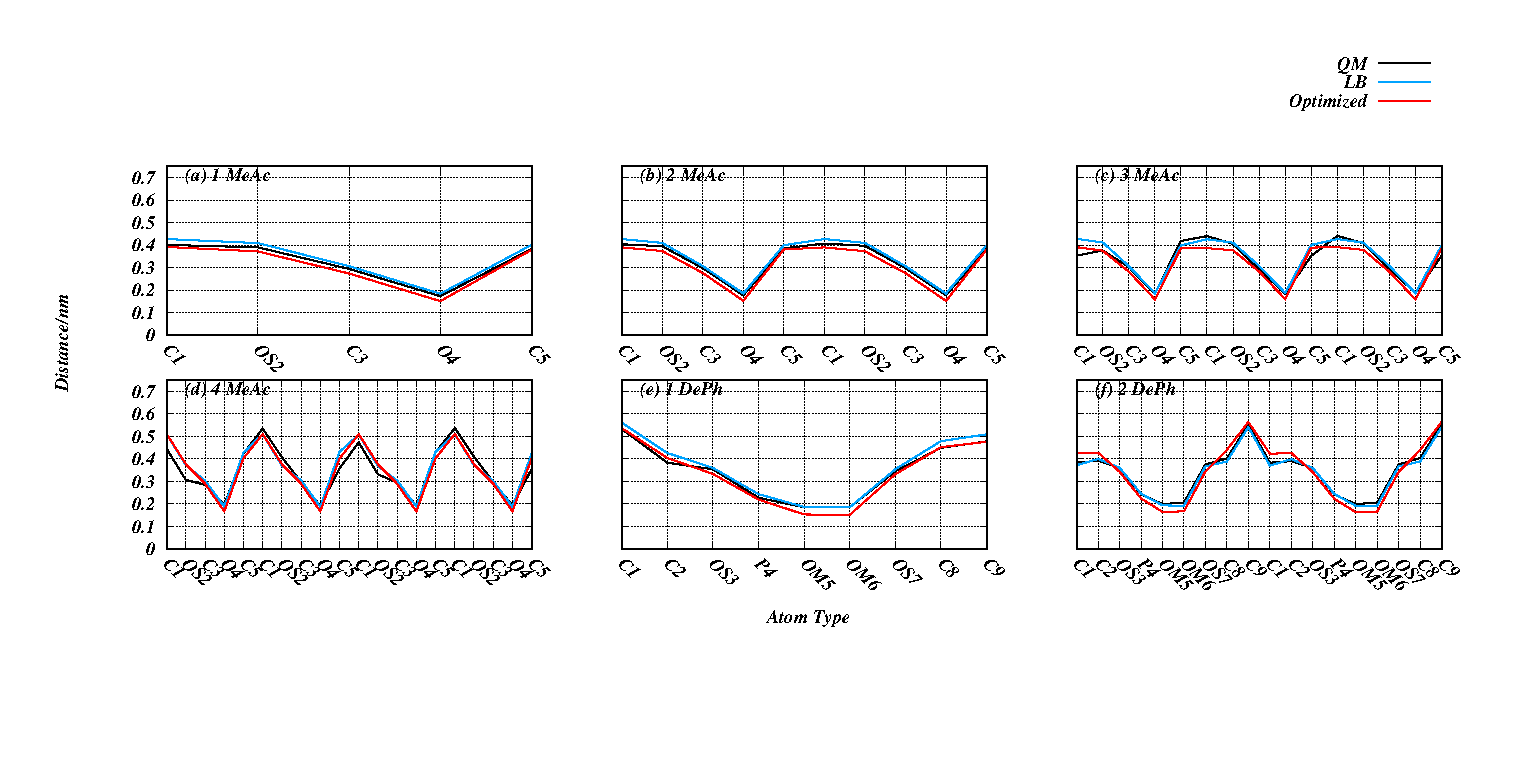
\includegraphics[width=\textwidth]{Figure_S2.eps}
\end{figure}

Describing the interactions of \mg with water presents several challenges, and there are numerous
models developed to describe \mg--water interaction~\cite{merzparams,villaparams,microparams}.
These models are optimized to improve the hydration free energies as well as
binding energies with various solvent models~\cite{merzparams,villaparams,microparams}.  
Previous work by our group has examined \mg models
from Li \etal{} and Allner \etal{}~\cite{merzparams,villaparams} in simulations with POPC lipids~\cite{kruczek:2019}, 
and found little variation among them in terms of their effects on lipid bilayer properties. 
With this in mind, we chose to focus our work here on the parameters developed by Li \etal{} because
their optimization procedures closely follow our focus on binding energies.
In recent work it has been reported that the existing \mg parameters, 
including those developed by Li \etal{}
overestimate the residence time for a water molecule in the 
first coordination shell of an ion~\cite{microparams}. 
In our past works using this force-field we reported 
insignificant Langmuir type adsorption of \mg ions to the POPC bilayer,
with waters retained in the first coordination shell of the ion~\cite{kruczek:2019}. 
We have also performed simulations with the parameters developed by Grotz \etal{} that directly
reduce residence times while not significantly changing other solvation 
properties of the ion~\cite{grotz:2021:optimized,microparams}. 
This was done to study how the interactions with water
could affect the first-shell coordination of \mg in the bilayer interface. 
We have {computed} 
the interaction cross-term for the \mg ion from Grotz \etal{}
with SPC/E water explicitly, using {the Lorentz-Berthelot mixing rules.}
Similarly to \li{}, we selected LJ cross-terms for use in our simulation following the procedure from Saunders \etal{} 2022~\cite{saunders:2022}. Target QM data for clusters of water with \mg are shown in table~\ref{tabch3:ionwater}.
\begin{table}[H]
    \centering
    \tiny
    \begin{tabularx}{\textwidth}{X|X|X|X|X|X|X}
        \hline
        Waters & CCSD(T)/CBS~\cite{wineman:2020:transferable} & PBE0+vdW~\cite{wineman:2020:transferable} & AMOEBA-HFC~\cite{wineman:2020:transferable} & Li et al.~\cite{merzparams} & Grotz et al.~\cite{microparams}  & Allner \etal{} \cite{villaparams}\\
        \hline
             1  &  -344.8  &  -349.9  &  -349.8  &  -276.8  & -282.8   &-270.3\\
             2  &  -651.0  &  -657.6  &  -657.3  &  -544.3  & -557.3   &-531.5\\
             3  &  -898.7  &  -904.6  &  -902.5  &  -792.1. & -815.2   &-774.3\\
             4  & -1101.2  & -1103.4  & -1100.4  & -1018.3 & -1055.3   &-995.7\\
        MAE &     -        &  4.9       &  4.0        &  91.1     &  71.3& 106.0     \\
        \hline
    \end{tabularx}
        \caption[\mg binding energies to water]{Mg$^{2+}$ binding energies to water clusters determined using different QM
    theories and classical force fields. All energies are in kJ/mol. These are used when
    computing the energies of substitution from water to lipid parts, which we use
    as our optimization target when selecting LJ cross-terms.}
    \label{tabch3:ionwater}
\end{table}
These energies for water were similar enough across force-fields that we chose to use only the values from Li \etal{}~\cite{merzparams} for use in computing substitution energies for our target data.
The result of our parameter search are shown in table~\ref{tabch3:params}.
\begin{table}
\tiny{
    \begin{tabularx}{\textwidth}{|X|X|X|X|X|X|X|X|X|X|X|}\hline
        \multirow{3}{*}{Atom type} & \multicolumn{4}{c|}{\li{}} & \multicolumn{6}{c|}{\mg} \\\cline{2-11}
                  &\multicolumn{2}{c|}{LB-Rules}&\multicolumn{2}{c|}{\mbnbfix}&\multicolumn{2}{c|}{LB-Rules}&\multicolumn{2}{c|}{\mbnbfix}&\multicolumn{2}{c|}{\mbnbfixmicro}\\\cline{2-11}
                  & \eps  & \sig  & \eps & \sig & \eps& \sig & \eps& \sig & \eps& \sig \\\hline
            CH3   & 1.07485 & 0.25797 & 0.99872 & 0.30898 & 0.19239 & 0.30856 & 0.68709 & 0.14257& 0.68709 & 0.14257\\\hline
            CH2   & 0.75411 & 0.27432 & 1.05729 & 0.20001 & 0.13238 & 0.32468 & 0.63126 & 0.20617& 0.63126 & 0.20617\\\hline
            OA    & 1.09408 & 0.21821 & 2.91925 & 0.20020 & 0.19044 & 0.26890 & 5.05190 & 0.26223& 5.05190 & 0.26223\\\hline
            P     & 1.85667 & 0.23975 & 6.99324 & 0.21844 & 0.32318 & 0.29044 & 3.89200 & 0.27811& 3.89200 & 0.27811\\\hline
            OM*   & 1.19328 & 0.21400 & 0.23749 & 0.20015 & 0.20771 & 0.26469 & 3.22262 & 0.17691& 3.22262 & 0.17691\\\hline
            CO*   & 0.35344 & 0.29727 & 0.48204 & 0.35920 & 0.06152 & 0.34796 & 0.56152 & 0.37127& 0.56152 & 0.37127\\\hline
            O*    & 1.19328 & 0.21400 & 0.06248 & 0.20068 & 0.20771 & 0.26469 & 2.43058 & 0.13069& 2.43058 & 0.13069\\\hline
            OW    & 0.95709 & 0.22875 & 0.95709 & 0.22875 & 0.16659 & 0.27944 & 0.16659 & 0.27944& 13.75000& 0.21010\\\hline
    \end{tabularx}}
    \caption[Lennard-Jones cross-terms for \mg]{Lennard-Jones cross-terms used in each \mg simulation. We have computed LB-terms using Lorentz-Berthelot (LB) mixing rules,
    starting with the self-terms for \li{} from Joung and Chetatham III\etal{}~\cite{joung:2008} and the self terms from \mg from the work of
    Li \etal{} ~\cite{merzparams}. The \mbnbfix parameters are chosen following the method described in section~\ref{sec:params}.
    The \mbnbfixmicro parameters for \mg only change the cross-term for OW-\mg, and were computed using LB-rules to mix the self-terms from
    Grotz \etal{}~\cite{microparams} with those of SPC/E water, without changing the cross-terms with anything else in the system. \eps~are in
    units of / Kj/mol and \sig~are presented in units of /nm.}
    \label{tabch3:params}
\end{table}
\section{Results and Discussion}
\subsection{Bilayer simulations of \li{} and \mg{}}
\subsubsection{Lipid bilayer structure}
% \paragraph{Densities}
The distribution of electron dense and heavy atoms is often studied by using
scattering techniques, like small-angle x-ray and neutron scattering. 
These methods
yield a scattering form-factor.  Densities can be obtained from the form-factor by solving
the inverse problem, which is a technically hard problem. In experiments this is usually solved by fitting a model to the form-factor.
Simulations give us direct access to atomic positions, and consequently
the densities. This allows us to compute a scattering form-factor by taking a cosine transform of the density{. The computed
form-factor}
can be compared with the direct measurements of the experiment.
The simulated lipid bilayer x-ray scattering form-factors and associated 
electron densities for each system are shown in figure~\ref{figch3:eledens}.
\begin{figure}[h!tb]
    \caption[Comparison of SAXS formfactors]{Comparison of x-ray scattering formfactors (a,b) and associated electron densities (c,d) for simulated systems. 
    {The system with \li{}{} salt has a slightly thicker bilayer compared to \na and the simulation without salt (a,c) and},
    \mg does not significantly change the bilayer thickness
    under any parameter set studied (b,d). }
    \label{figch3:eledens}
    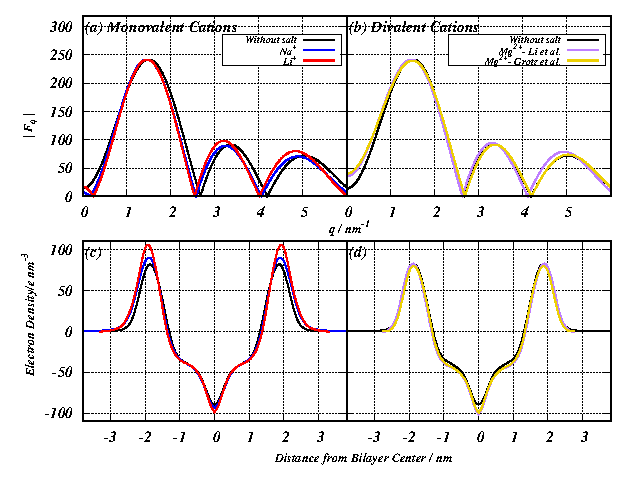
\includegraphics[height=0.3\textheight]{Figure_1.eps}
\end{figure}
We compare all form-factors for each system to that of a system simulated without salt, published
in our previous work~\cite{kruczek:2017}.
The bilayer thickness \dhh~is determined by measuring the distance between the
peaks in the electron density, which roughly localize the electron-dense phosphates in the
lipid headgroup -- the values for this can be seen in table~\ref{tabch3:struc}.
\begin{table}
    \caption[Bilayer simulation details and structure]{Bilayer simulation details, and structural parameters. Here we detail the various
    structural measurements of each simulated bilayer.
    \dhh~ is the distance measured between the peaks in the electron density, which localize the electron-dense phosphate moiety in the lipid headgroup.
    \db~ is a distance between the Gibb's surfaces{\cite{fogarty:2015}} on the probability density of solvent as it approaches the lipid bilayer.
    \dc~ is the distance between the Gibb's surfaces on the probability density of lipid chains, and represents the lipid chain thickness.
    Volume per lipid \vl~ is measured by dividing the volume of the entire system into solvent and ions, and lipid following the method by Petrache \etal{}
    {\cite{petrache:1997}}.
    This \vl~ is the sum of the \vh~ and V\textsubscript{C}, which are the volume per lipid headgroup and volume per lipid chains respectively.
    Area per lipid molecule \al~ is computed as the ratio of twice the lipid chain volume \vc~ with \dc. We also report the
position of the hydration boundary of each system, which we compute as the point where the second water order parameter $P_2(cos(\beta))\approx 0$
{as was done in Saunders \etal{} 2019~\cite{saunders:2019}}.}
    \label{tabch3:struc}
    {\tiny
    \begin{tabularx}{\textwidth}{Y|Y|Y|Y|Y|Y}
            &No Salt&\na&\li{}&\mgmbnbfix&\mgmicro\\\hline
        \dhh (nm)    &3.744   $\pm$ 0.107  &3.764   $\pm$ 0.088 &3.864  $\pm$ 0.070&3.832  $\pm$ 0.364  &3.768  $\pm$ 0.525\\
        \db  (nm)    &3.654   $\pm$ 0.047  &3.936   $\pm$ 0.043 &4.511  $\pm$ 0.048&4.325  $\pm$ 0.044  &4.213  $\pm$ 0.049\\
        \dc  (nm)    &2.707   $\pm$ 0.034  &2.897   $\pm$ 0.034 &3.015  $\pm$ 0.034&2.880  $\pm$ 0.029  &2.809  $\pm$ 0.032\\
        \vl  ($\times 10^{-3}\text{nm}^3$)&1215.57 $\pm$ 1.0   &1211.32 $\pm$ 1.21 &1201.2 $\pm$ 1.05&1219.8 $\pm$ 1.24  &1227.7 $\pm$ 1.24\\
        \vh  ($\times 10^{-3}\text{nm}^3$)&310.68  $\pm$ 1.14  &314.81  $\pm$ 0.75 &306.0  $\pm$ 1.01&324.0  $\pm$ 1.26  &327.9  $\pm$ 1.10\\
        \vc  ($\times 10^{-3}\text{nm}^3$)&904.89  $\pm$ 1.28  &896.50  $\pm$ 1.19 &895.3  $\pm$ 0.91&895.8  $\pm$ 1.05  &899.8  $\pm$ 1.06\\
        \al  ($\times 10^{-2}\text{nm}^2$)&66.86   $\pm$ 0.85  &61.89   $\pm$ 0.73 &59.39  $\pm$ 0.69&62.21  $\pm$ 0.63  &64.35  $\pm$ 0.82\\
        Hydration Boundary (nm) & 2.79 &3.69&3.63 &3.48&3.33  \\
\end{tabularx}}
\end{table}

Experiments often report various types of thicknesses, volumes, and cross-sectional areas that are model dependent.
We also compute these quantities to compare the simulation results with experiments. These values are presented in 
table~\ref{tabch3:struc}.
Based on the \dhh~and the \dc~ there is a slight thickening 
of the bilayer in the \li{} {simulation} above that seen in the \na {simulation}.
The \mg simulations {, irrespective of the parameter set, yield} much less thickening than {the}  
Li\textsuperscript{+} {simulation.} 
{The volumes per lipid (\vl), headgroup (\vh), and chains (\vc) are computed using the method of
Petrache \etal{}~\cite{petrache:1997}. This is done by optimizing the function:
\begin{equation}
    \label{eq:volumeobj}
    \Omega(v_i)=\sum^{\rho_s}_{z_j}(1-\sum^{N_{\text{Groups}}}_{i=1}{(\rho_i(z_j)v_i)^2})\text{,}
\end{equation}
where $\rho_i(z_j)$ is the number density of the $i$ component in the
$z_j$ slice of the box and $v_i$ is the corresponding partial component volume. $N_\text{Groups}$ is the number
of atom groups for which we are dividing the system volume into component volumes -- we have groups for solvent plus ions,
lipid chain without the terminal methyls (CH\textsubscript{*}), terminal methyls (CH\textsubscript{3}), and the lipid headgroups (H).
The lipid volumes are then computed as 
\begin{equation}
    \text{\vc}=N_{\text{CH}_*} \times v_{\text{CH}_*}+N_{\text{CH}_3} \times v_{\text{CH\textsubscript{3}}}
\end{equation}
and
\begin{equation}
    \text{\vh}=N_{H} \times v_{\text{headgroup}}\text{,}
\end{equation}
where $N_{\text{CH}_*}=30$, $N_{\text{CH}_3}=2$, $N_{\text{H}}=20$ are the number of united atoms per atom group for CH\textsubscript{*},
CH\textsubscript{3}, and H.
}{
The chain volume \vc~ is similar for all systems studied, and there is some variation in the headgroup volume \vh~.
However, this method of dividing up the volume is more prone to errors in the headgroup region due to 
significant overlap between the headgroup and solvent densities. 
Thus, we also see similar variation in the total lipid volume \vl. 
}
The two-dimensional area per lipid \al~is defined as
{$\frac{2V_c}{2D_c}$ as is often reported from SAXS and SANS experiments~\cite{nagle:2000}, and is an important
measure of how the lipids condense as the bilayer thickens.}
{Both the simulations with \mg yield bilayers with a larger \al~ 
    than the monovalent ions studied in this work, and are closer
in area to the simulation without salt.
}

The detailed structure of molecules and their neighborhoods are often studied using 
various nuclear magnetic resonance (NMR) techniques.
{At present, these experiments with various salts are sparse.}
{Thus,} we report these data with anticipation that future experiments will fill this gap and validate
or invalidate
these numbers.
Lipid chain ordering is determined via the acyl chain $S_{CD}$ per carbon
atom. These can be seen in figure~\ref{figch3:op}. 
\begin{figure}[h!tb]
    \caption[Acyl chain order parameters]{Acyl chain carbon-deuterium order parameters. These are computed for the Sn1 and Sn2 chains of each lipid starting at the 
        second carbon in the chain\cite{egberts:1988,Douliez:1995}. We note that the lipids simulated in systems of monovalent ions (a,c) show a significant increase
in the lipid chain ordering for both acyl chains. The systems simulated with \mg (b,d) are much closer in ordering to that of a system
simulated without ions.}
    \label{figch3:op}
    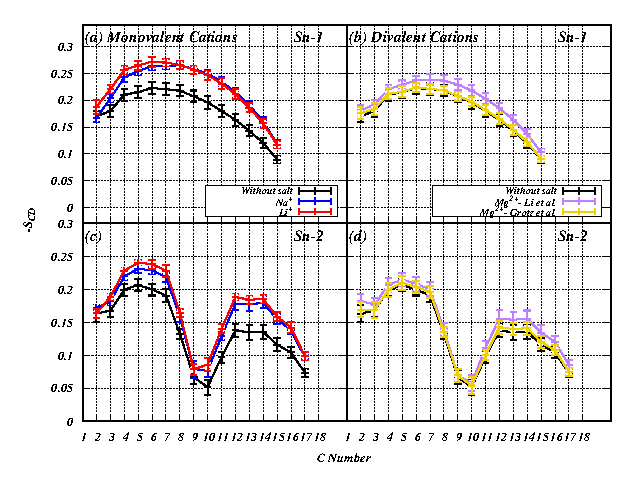
\includegraphics{Figure_2.eps}
\end{figure}

There is significant increase in chain ordering in the systems 
with \na and Li\textsuperscript{+}, which {is} consistent with the slight thickening
of the bilayer seen in the \db~ values. The less coordinated \mg systems have remained much closer to the 
ordering seen in the no-salt simulation.


\section{Specific ion adsorption}
\subsection{Bulk ions}

Interfaces in salt solutions give rise to a double layer of cations and anions at the surface~\cite{israelachvili:2011:intermol}. 
Ions in these double layers get stuck to the surface, or adsorb, which is sometimes referred to as specific binding. Zwitterionic lipid bilayers have no net charge before ions are adsorbed,
so this adsorption
determines the surface charge density on the substrate. This charge is measured experimentally using the electrophoretic mobility of the vesicle. Interpretation
of such experiments requires one to define a surface, often called the ``slip-surface'' where solvent 
beyond that point
can be represented by a dielectric continuum. The electrostatic potential at this surface is the $\zeta$--potential.
In simulations the interface is not a simple surface, but a region {without a clear point of delineation}. 

\subsubsection{Hydration boundary}
We {identify} this 
slip-surface boundary as the point where 
water orientational ordering is negligible, i.e.
beyond the ``slip-surface'' 
boundary water {quadrupoles} are {sufficiently isotropic,
giving dielectric properties of water similar to that of bulk solvent}.
We compute this by first dividing the box into 
slices along the direction normal to the bilayer. 
For each water within a slice we 
compute the average value of first and second order legendre polynomial of 
the cosine of the angle between the box z-axis and
the water O-H bond vector, and then average these values over the last 150 ns of simulated time.
Figure~\ref{figch3:h2order}~shows the water order parameters 
as a function of the distance of a slice from the bilayer center.
\begin{figure}[h!tb]
    \caption[Water orientational order parameters]{Water order parameters.   
        {The P1 and P2 calculated for monovalent cations (a,c) show greater 
            organization in the bulk region and the B\textsubscript{-2} regions, and less organization within 
            the lipid-occupied regions of the system (B\textsubscript{+} and B\textsubscript{-1}) compared to the simulation without salt. 
        } 
{On the other hand, with the presence of \mg salts we observe an overall less pronounced effect in the
bulk and B\textsubscript{-2} regions compared to the system without salt (b,d).}
}
    
    \label{figch3:h2order}
    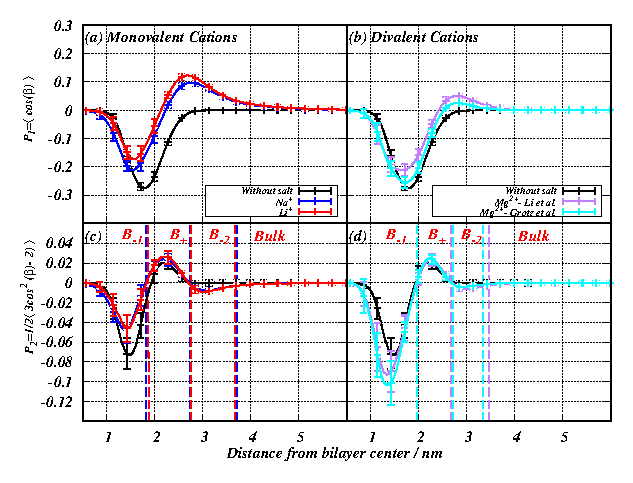
\includegraphics[width=0.5\textwidth]{Figure_3.eps}
\end{figure}

The first order parameter describes the in-out ordering of the bond vector with respect to the 
box z-axis -- a vector parallel to the axis and pointing normal to the bilayer would have a positive
ordering, and a vector pointing into the bilayer would have a negative ordering. We see that waters at the surface
of each bilayer have a significant outward orientation at the bilayer surface, and that reverses as we move
closer to the bilayer center. When compared to the system simulated without ions, we see that
the monovalent ions perturb the water in-out orientation 
more than Mg\textsuperscript{2+}, especially in the case of the \mgmicro
parameters.

The second order parameter
roughly describes the organization of the quadrupole moments of water, {and the value of this parameter
can be used to compute the} quadrupolar splitting values determined in 
deuterated water NMR experiments~\cite{aaman:2003,kruczek:2017:ether}.
The vertical dotted lines in figure~\ref{figch3:h2order} denote regions of interest in the bilayer 
based on the {sign} of the second order parameter. We call the innermost region of negative ordering
B$_{-1}$, which ends when the values become positive. This next region of positive ordering is
called B$_{+}$, and the following region of negative ordering is B$_{-2}$. Each bilayer system with ions
has these regions, but they are at differing distances from the bilayer center.
It should be noted that beyond the $B_{-2}$ region the ordering does not abruptly reach zero in the systems
simulated with salt.

{
    Figure~\ref{figch3:h2order} shows monovalent ions have 
    less organization in the B\textsubscript{-1} region (inside the lipid headgroup) when compared to that of the divalent ions,  
    whereas in regions B\textsubscript{+} and B\textsubscript{-2} (closer to the bilayer surface) the divalent ions show significantly
    less organization compared to that of monovalent salts.} 
The hydration boundary is determined by  
fitting an exponential decay to the second water order parameter starting
at the minimum of the B$_{-2}$ of the histogram.
The decay length is used to demarcate the point where the ordering becomes zero -- water beyond this region is
regarded as bulk solvent. The location of the hydration boundary 
is noted in figure~\ref{figch3:h2order}, and the distance 
to this point from the bilayer center is listed in table~\ref{tabch3:struc}.

\subsubsection{Poission-Boltzmann Theory}
With the boundary defined, we look to the region of bulk solvent to examine the behavior of ions and ascertain that
they follow the predictions of PB-theory\cite{israelachvili:2011:intermol}. 
The purpose of this endeavor is to distinguish the ions in bulk solvent from those that are adsorbed,
as the density of the adsorbed ions are expected to deviate from PB-theory predictions.
We must first compute all the model parameters for the number density and electrostatic potential predicted by
PB-theory, and compare our simulation results to this prediction.
The PB-theory assumes 
that the number density of ions follow a Boltzmann distribution:
\begin{equation}
    \rho(z) = \rho_0 \exp\big({- \bar z \text{\si{\elementarycharge}} \beta \psi(z)}\big)\text{,}
    \label{eq:gcnum}
\end{equation}
where $\rho_0$ is the ion density in the center of the dielectric continuum, $\bar z$ is the valency of the ion, 
$\beta = (k_bT)^{-1}$, \si{\elementarycharge} is the charge
on an electron, and $\psi(z)$ is the electrostatic potential. The surface is defined by the hydration boundary of each system. 
The lengths of the solvent occupied regions, $D$, {in each system is} found by measuring the distance across the solvent from the 
hydration boundary of one leaflet of the bilayer to the other. 
These values are listed in table~\ref{tabch3:gctheory}.
\begin{table}
    \caption[Poisson-boltzmann theory parameters]{Poisson-boltzmann theory parameters. These parameters are computed for each
    simulated system studied (excepting the bulk density $(\rho_{0,i})$, 
    which we fit to our simulation results). These are then used to compute the
    number density distribution and the electrostatic potential as described by 
    Poisson-Boltzmann theory to compare to our simulation results.
    \sig is the surface charge density of the bilayer, D is the length
    of the bulk-solvent occupied region of the box, K is the Debye
    screening length, and $\rho_{0,i}$ is the number density of the particular 
    ion at the center of bulk solvent.}
    \label{tabch3:gctheory}
    \begin{tabularx}{\textwidth}{|X|X|X|X|X|}\hline
        Parameter                    & \na  & \li{}    & \mgmbnbfix    & \mgmicro \\\hline
        \sig ($e/nm^{2}$)            &0.161 &0.182   &0.0690  &0.0476     \\\hline
        D~($nm$)                     &26.927&26.557  &26.658  &25.226     \\\hline
        K~($nm^{-1}$)                &3.331 &3.333   &3.913   &3.921      \\\hline
        $\rho_{0,cation}$~($nm^{-3})$&0.059 &0.060   &0.091   &0.092      \\\hline
        $\rho_{0,anion}$~($nm^{-3})$ &0.062 &0.063   &0.183   &0.185      \\\hline
    \end{tabularx}
\end{table}
This places the surfaces at $z=\pm D/2$~nm, where $z=0$ is the center of the solvent-occupied region of the simulation box.
The electrostatic potential $\psi(z)$ is modeled as a sum between two Debye-Huckle potentials~\cite{israelachvili:2011:intermol}:
\begin{align}
    &\psi_{1}(z) = \psi_s \exp\bigg({-K(z+\frac{D}{2})}\bigg)\\
    &\psi_{2}(z) = \psi_s \exp\bigg({K(z-\frac{D}{2})}\bigg)\\
    \label{eq:gcpot}
    &\psi(z) = \psi_1(z) + \psi_2(z) - \big({\psi_1(0)+\psi_2(0)}\big)\text{,}
\end{align}
where $\psi_s = \frac{\sigma}{\epsilon_0\epsilon} K$ is the electrostatic potential at the bilayer surface
as defined by the hydration boundary, $\epsilon$ 
is the dielectric constant of SPC/E water $\epsilon=70.7$~\cite{reddy:1989:dielectric}, and $\sigma$
is the surface charge density of the bilayer leaflet~\cite{israelachvili:2011:intermol}. 

$\sigma$ is determined for
each system by integrating the charge density of all species within the hydration boundary on either side of the bilayer.
This charge divided by the box area is the surface charge density.
These values can be seen in table~\ref{tabch3:gctheory}. {Since our
    phospholipid is zwitterionic, all of the surface charge comes from the
ions that have accumulated within 
the hydration boundary (see figure~\ref{figch3:dens})}
\begin{figure}[h!tb]
    \caption[Number densities]{Number density of lipid headgroup species and
    ions near the bilayer interface. (a-b) We report that the 
    monovalent cations show peaks near the phosphate, with
    accumulation of an anion peak that resembles the double layer.
    (c-d) \mg does not show significant accumulation in the 
    lipid bilayer headgroup compared to the monovalent ions,
    with a similarly small anion peak. However, in all systems
    studied, ions are accumulated near the phosphorus.
    Integrating the number density of cations within the hydration boundary,
    denoted by the purple vertical dashed line, gives the number of ions that are
    sterically bound. The orange vertical dashed line delineates the \dhh~and the 
    red vertical dashes
delineate the D\textsubscript{C}~of the bilayer.}
    \label{figch3:dens}
    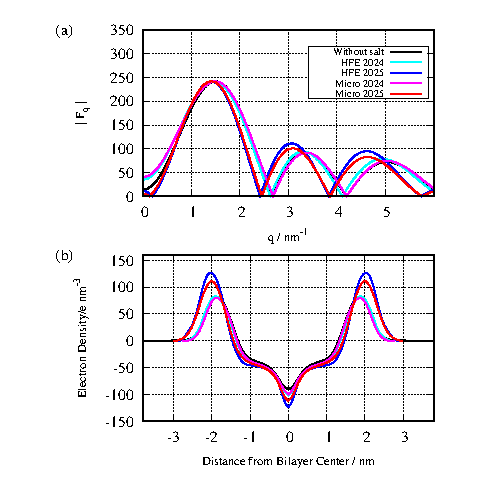
\includegraphics[width=\textwidth]{Figure_4.eps}
\end{figure}

Returning to equation~\ref{eq:gcpot}, $K$ is the inverse Debye length,
\begin{equation}
K=\sqrt{\sum_{i} \rho_{0,i} \bar z_i^2\frac{\text{\si{\elementarycharge}}^2}{\epsilon_0 \epsilon k_bT}},
\label{eq:debyelength}
\end{equation}
where $\rho_{0,i}$ is the density of each ion in a given system at the center of bulk solvent.
This is taken as an average of the number density of each ion in the solvent occupied region of the box.

Finally, we fit equation~\ref{eq:gcnum} to the density of anions in 
bulk solvent via $\rho_0$. The comparisons
can be seen in figure \ref{figch3:catgcdens}.
\begin{figure}[h!tb]
    \caption[Number densities of cations and anions]{Number density of cations and anions in the bulk solvent-occupied region of each
    simulated system, compared with theoretical predictions from PB-theory for each calculated $\sigma$. PB-theory predictions
    correspond well with the simulation results within the region bounded by the hydration boundary.}
    \label{figch3:catgcdens}
    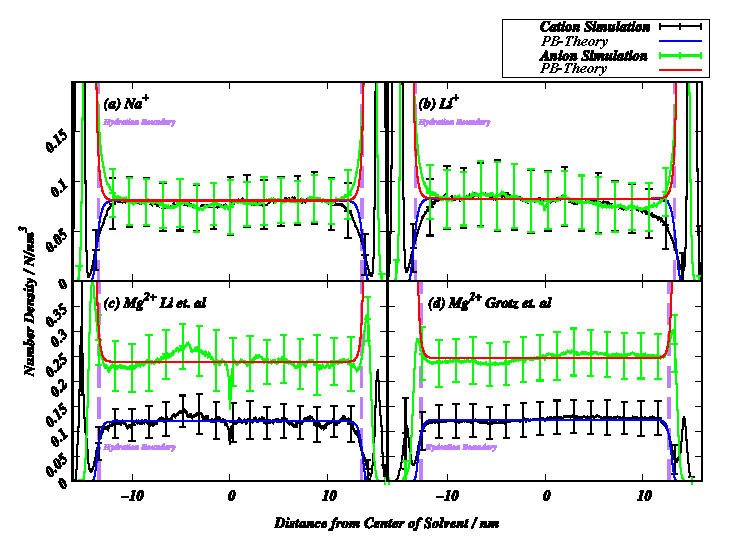
\includegraphics[width=\textwidth]{Figure_5.eps}
\end{figure}
Past the hydration boundary of the lipid bilayer, it can be seen that the density of anions continues 
to climb monotonically. Additionally, the density of cations 
drops monotonically to a trough value before climbing closer to the bilayer center, near the phosphate groups 
(see figure \ref{figch3:dens} and \ref{figch3:catgcdens}). 


We also compare {the} 
electrostatic potential from our simulations 
to the potential from PB-theory 
(figure \ref{figch3:potgc}). 
\begin{figure}[h!tb]
    \caption[Electrostatic potential]{Electrostatic potential in the bulk solvent-occupied region compared to predictions from PB-theory. We report good
    agreement between the theoretical potential shown in green, and the simulation results shown in black, within the region bounded by the hydration
    bounds of the lipid bilayer.}
    \label{figch3:potgc}
    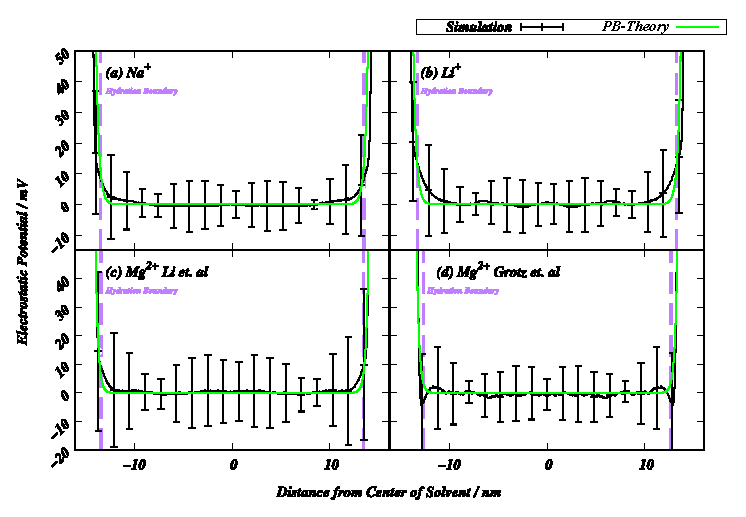
\includegraphics[width=\textwidth]{Figure_6.eps}
\end{figure}
The electrostatic potential for each simulated system can be computed 
by twice integrating the Poisson equation 
\begin{equation}
    \phi(z)=-\frac{1}{\epsilon_0}\int_{0}^{z}\int_{0}^{z'}\rho(z) dz dz' + C_1z + C_2\text{.}
    \label{eq:poissonint}
\end{equation}
We set the boundary conditions that
the electric field in bulk solvent must be zero, and the electrostatic potential at the box edge must be zero.
The electrostatic potential from simulation agrees well with the prediction from PB-theory.


\subsection{Adsorbed ions}
\label{sec:boundions}
The total number of adsorbed ions are counted as the number of ions within the ``slip-surface'' or ``hydration-boundary'' of the bilayer, and
further characterization is based on the level of hydration of the ion.
Binding constants from the Langmuir Isotherm model are often computed in experiments to describe ion binding affinity for
surfaces; however, this model requires a fixed number of binding sites per lipid. The actual number of binding sites
per lipid is not known. Therefore, we report the number of ions adsorbed per lipid $(\theta)$, which 
{is related to} 
the binding affinity of each ion for the lipid bilayer.
We observe 0.51 \na per lipid bound, 0.57 \li{} per lipid, 0.13 \mg per lipid in the \mgmbnbfix system, and 0.10 \mg per lipid
in the \mgmicro system. We see a substantially larger number of \na and \li{} adsorbed per lipid than
\mg, which may be reflective of the amount of space occupied by each ion, and seems to follow the
binding modes such that the more dehydrated ions correlate with a larger number of ions adsorbed per lipid.
The fraction of cations adsorbed in each mode of adsorption can be seen in table~\ref{tabch3:cationfrac}, and the fractions
of \cl anions adsorbed can be seen in table~\ref{tabch3:anionfrac}.
\begin{table}
    \caption[Fractions per lipid of cations per adsorption mode]{Fractions per lipid of cations perfectly adsorbed, imperfectly adsorbed, sterically adsorbed, and non-adsorbed cations
        {averaged over the last 150~ns of simulation time}. These are computed
    by counting the number of waters in the first-coordination shell of every ion in the simulation box in every frame. For the total number
    of adsorbed ions, we
    only check if the ion is within the hydration boundary of the bilayer. We then subtract the number within this region that are
    completely dehydrated -- these are the perfectly adsorbed ions. We further subtract any ions that have lost 
    one or more waters -- the imperfectly adsorbed
    ions. The remaining are considered sterically adsorbed. 
    We also report the total number of bound ions per lipid as a measure 
    of the affinity of the ion to the lipid bilayer -- the number of \mg
    ions per lipid is fall smaller than that for the more perfectly adsorbed ions \li{} and Na\textsuperscript{+}.}
    \label{tabch3:cationfrac}
    \begin{tabularx}{\textwidth}{|X|X|X|X|X|}\hline
    Adsorbed cations / lipid & \na & \li{} & \mgmbnbfix   & \mgmicro \\\hline
    Total     $\theta$       &{0.472}&{0.575}&{0.129}&{0.091}     \\\hline
    Steric    $\theta_s$     &{0.010}&{0.015}&{0.116}&{0.071}     \\\hline
    Imperfect $\theta_I$     &{0.068}&{0.165}&{0.008}&{0.020}     \\\hline
    Perfect   $\theta_P$     &{0.394}&{0.395}&{0.005}&{0.000}     \\\hline
    \end{tabularx}
\end{table}
\begin{table}
    \caption[Fractions per lipid of anions per adsorption modality]{Fractions per lipid of anions perfectly adsorbed, imperfectly adsorbed, sterically adsorbed, and non-adsorbed anions in each simulation, defined in the same way as we define
    adsorption of cations. These are computed
    by counting the number of waters in the first-coordination shell of every anion in the simulation box in every frame. For the total number
    of adsorbed anions, we
    only check if the anion is within the hydration boundary of the bilayer. We then subtract the number within this region that are
    completely dehydrated -- these are the perfectly adsorbed anions. We futher subtract any ions that have lost
    one or more waters -- the imperfectly adsorbed
    ions. The remaining are considered sterically adsorbed. We indicate each system by the cation name, as the anion in the system is always Cl\textsuperscript{-}.
    We note that the anion binding fractions follow the trend seen in the total number of cations bound for each system, due to the formation of the ionic double-layer
    at the bilayer-water interface.
    Most anions adsorb sterically in each system, with some adsorbing imperfectly as they approach the positively charged choline trimethylammonium in the lipid headgroup.}
    \label{tabch3:anionfrac}\tiny
    \begin{tabularx}{\textwidth}{|X|X|X|X|X|}\hline
    Adsorbed anions / lipid     & \cl in \na System & \cl in \li{} System & \cl in \mgmbnbfix System& \cl in \mgmicro System\\\hline
    Total      $\theta  $&0.423&0.463& 0.186&0.208 \\\hline
    Steric     $\theta_s$&0.209&0.213& 0.107&0.126 \\\hline
    Imperfect  $\theta_I$&0.214&0.250& 0.079&0.082 \\\hline
    Perfect    $\theta_P$&0.000&0.000&  0.0 & 0.0  \\\hline

    \end{tabularx}
\end{table}
\cl adsorption fractions follow a similar trend to that of the total number of cations bound, but adsorption
is almost entirely in the steric modality.




\subsubsection{Adsorption modalities}

% The total number of adsorbed ions can be seen in~\ref{tabch3:struc}.
Further characterization of the adsorbed ions begins by examining the first-shell coordination partners of cations in each system.
This can be counted by first determining a cutoff value for the first hydration shell of each ion 
-- the values for this cutoff are
3.2~\AA~for Na\textsuperscript{+}, 2.7~\AA~for Li\textsuperscript{+}, 3.3~\AA~for Mg\textsuperscript{2+}, 
and 3.0~\AA~for Cl\textsuperscript{-}. 
These values are determined from radial distribution 
functions for water oxygen (or water hydrogen in the case of \cl) around each. 
This cutoff is used to produce a neighborlist for ions
across each simulation in every frame, and count the number of neighbors within this cutoff. 
These data {are} histogrammed and averaged over
the last 150ns of simulation time. The results for this are presented in figure~\ref{figch3:cood}.
\begin{figure}[h!tb]
    \caption[First shell coordinators for \li{} and \mg]{First shell coordination partners 
        for \li{} and \mg in each simulation. 
        These are computed over the last 150ns of 
        simulation time in each system by counting 
        the atoms of each species within a cutoff 
        of each ion in the system, and histogramming 
        the data based on the position of the ion. 
        The dotted vertical lines denote the various 
        bilayer surfaces -- the vertical black
        line delineates the hydration boundary of the bilayer,
        the vertical blue line delineates the D\textsubscript{HH},
        and the vertical red line delineates the D\textsubscript{C}.
        \li{} (a) retains some water 
        coordination well into the bilayer
        interface.
        \mgmbnbfix (b) on the other hand does not lose
        nearly any first-shell coordinating
        waters in the bilayer, with some exchange for phosphate
        oxygens. The \mgmicro (c) parameters yield again more exchange but 
        relatively far less than the monovalent
    ions.}
    \label{figch3:cood}
    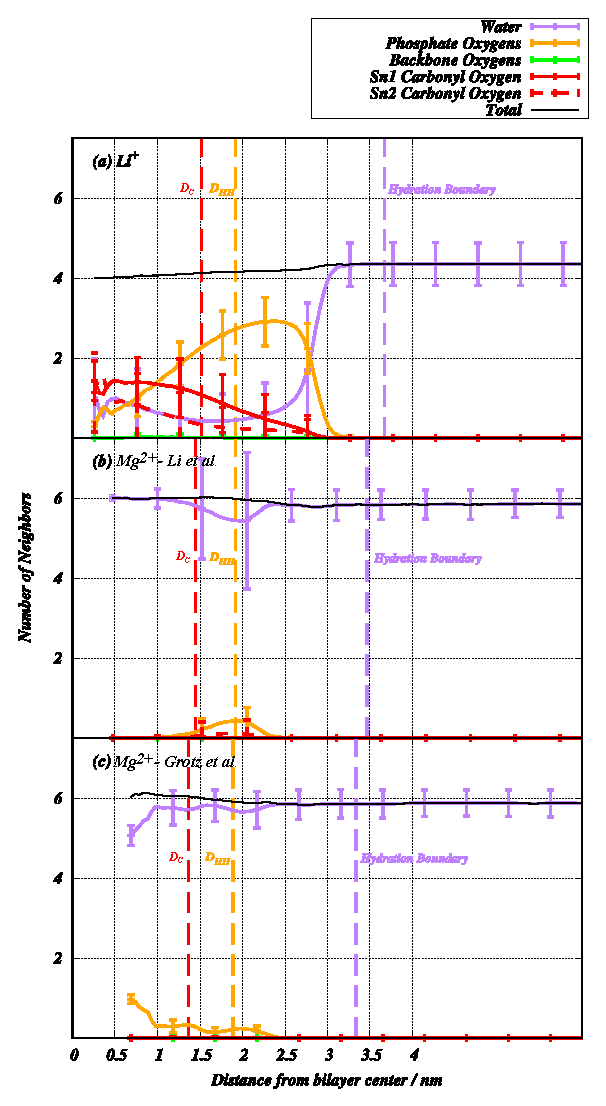
\includegraphics[height=0.7\textheight]{Figure_7.eps}
\end{figure}

The number of perfectly adsorbed ions is determined by counting the number of ions without any remaining 
waters in their first coordination shell. It is observed that in the \na system, a 
majority of the ions adsorbed to the bilayer are completely dehydrated. %(see table~\ref{tabch3:cationfrac}). 
The \li{} system has a similar fraction of perfectly adsorbed ions compared to Na\textsuperscript{+}, 
and practically no perfectly adsorbed 
ions are seen in any of the \mg simulations. \cl anions are not seen adsorbed perfectly in any simulation.

Similarly to the perfect adsorption case, imperfectly adsorbed ions are counted as ions with one or more waters in their 
first coordination shell, but missing at least one
water from the shell. {We use the number of coordinating waters of an ion in the bulk solvent region
    of our simulation as the maximum coordination number for the ion (Figure 7). This
gives a coordination number of 4 for \li{} and 6 for 
Mg\textsuperscript{2+}.} We calculate 
{the number of imperfectly adsorbed ions} by counting the number of ions with 
one or more water missing from their hydration shell, and then subtracting the number of perfectly adsorbed ions.
We see more than twice the fraction of these ions in the \li{} system compared to the \na system. \mg shows an insignificant
number of imperfectly adsorbed ions. \cl adsorbs in a large fraction imperfectly, as they begin to interact with the headgroup trimethylammonium.

The remaining ions are considered sterically adsorbed -- this number is whatever ions remain after subtracting the 
perfect and imperfectly adsorbed ions from the number of overall adsorbed ions based on the position of the hydration boundary. 
\mg seems to have most of the ions in this adsorption mode, where \na and \li{} do not 
adsorb in this way in significant numbers. Additionally, \cl shows significant steric adsorption.

These data raise the question, what determines the mode of adsorption for a given ion? Since everything else, such as
the substrate and the solvent, are held constant, the magnitude of the electric field at the position of the hydration shell
of each ion is all that remains to determine the adsorption modality of the ion (figure~\ref{figch3:cationfrac}).
\begin{figure}[h!tb]
    \caption[Fractions of ion-adsorption modalities]{Fractions of ion-adsorption modality per each simulated system as a function of electric field strength. Here we 
    show that the fractions of ions adsorbed in each modality follow a trend with an increasing electric field strength at the
    hydration shell of the cation. The overall trend is that the cations with the weakest field at the hydration shell position
    adsorb more perfectly, and as the field strength increases more ions adsorb imperfectly and then sterically. We note
    that little correlation with field strength can be seen in the total number adsorbed per ion.}
    \label{figch3:cationfrac}
    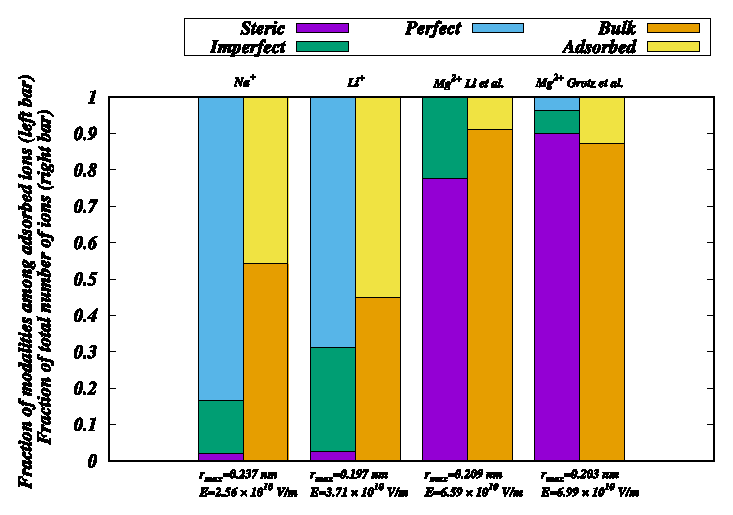
\includegraphics{Figure_8.eps}
\end{figure}
The electric field strength of each ion is calculated by applying Coulomb's law to a point charge, placing the test charge at the 
position of the first hydration shell of the ion in question. We note that the \mgmbnbfix ion keeps waters slightly closer in the hydration shell
compared to the \mgmicro model{,}{resulting in} a stronger electric field 
produced at this point by that ion.
The largest ion with the smallest charge-density \na dehydrates completely in the largest fraction. \li{} is smaller, and thus the field near
the first shell is stronger and can hold waters a little better than \na. \mg is similar in size to \li{}, but has a 2+ charge and
holds onto waters substantially more than either of the monovalent ions.  
We also note that the $\norm{\vec{E}}$ does not exhibit strong correlation with the fraction of the total number of ions adsorbed in each system, it
only determines the adsorption mode. 

\section{Conclusions}
Ion adsorption to porous interfaces is a complex interplay 
between solvent--surface, solvent--ion, and solvent--solvent
interactions. With the solvent--surface and solvent--solvent interactions 
held constant, we identify
three different adsorption modalities of ions based on the degree of 
dehydration of the ion upon adsorption. 
The binding modality of a particular ion is significantly correlated 
with the electric field strength of the ion
at the position of the first hydration shell, with stronger fields 
encouraging less dehydration of the ion upon
adsorption to the surface {(figure 8)}. This affect appears irrespective of the force-field 
used in the case
of \mg, which primarily adsorbs in the non-Langmuir type steric modality.


Furthermore, we identify several bilayer structural
parameters that can be verified experimentally via x-ray scattering, neutron
scattering,
or various NMR methods {(figures 1, 2, and 3 respectively).}
While the effect on lipid bilayer structure is not obvious in
the electron density {(figure 1)}, the pertubation can be seen in the \db~and water density --
the less hydrated ions induce slight thickening of the lipid bilayer. This
is reinforced by the chain ordering, where these ions increase chain ordering {(figure 2)} 
while the hydrated ions leave the lipid bilayer structure similar to that of the no-salt case.
These two results can be verified experimentally via solvent deuterium NMR, and lipid chain NMR.
In the case of POPC, we expect deuterium solvent quadrupolar splitting values will be 
{larger} 
for the less hydrated ions \na and \li{} when compared to the more hydrated Mg\textsuperscript{2+} {(figure 3)}. 
We also expect the lipid chain order parameters to follow the opposite trend,
with the monovalent ions inducing more ordering and \mg inducing a smaller change from the no-salt system.
We also expect that the adsorption of \mg will be less detectable via the 
electrophoretic mobility of a vesicle in an MgCl salt solution, as
the energy required to remove a hydrated ion from 
beneath the slip-surface of a vesicle may be low enough to allow their escape, while a dehydrated ion may remain
adsorbed.
These experiments are needed to verify
these conclusions. 